%------------------------------------------------------------------------
\begin{frame}[fragile] \frametitle{\cello\ AMR philosophy}
\begin{itemize}
\enhance{1}\item AMR data structures required for multi-resolution
\enhance{2}\item Arrays are preferred for uniform resolution regions
\enhance{3}\item Issues with standard tree-based AMR
\begin{itemize}
\enhance{4}\item Lots of small patches at finest resolution
\enhance{5}\item $2^d$-tree refinement is too ``shallow'' for deep AMR
\end{itemize}
\enhance{6}\item Three proposed modifications
\begin{itemize}
\enhance{7}\item Patch coalescing
\enhance{8}\item Individual child refinement
\enhance{9}\item $k^d$ refinement with backfill
\end{itemize}
\end{itemize}
\end{frame}

\begin{frame}[fragile] \frametitle{Patch Coalescing}
\centerline{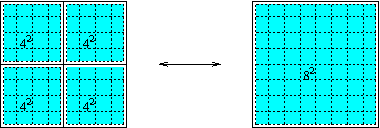
\includegraphics[width=2.5in]{coalesce.png}}
\begin{itemize}
\enhance{2}\item Replace AMR with larger arrays when possible
\enhance{3}\item Replace arrays with AMR when necessary
\enhance{4}\item Added flexibility can reduce AMR tree size
\end{itemize}
\end{frame}

\begin{frame}[fragile] \frametitle{Individual Child Refinement}
\centerline{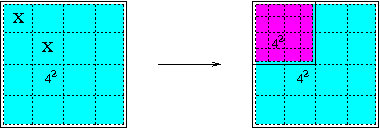
\includegraphics[width=2.5in]{amr-child.png}}
\begin{itemize}
\enhance{1}\item Refine children individually instead of all or nothing
\enhance{2}\item Added flexibility can reduce AMR tree size
\end{itemize}
\end{frame}

\begin{frame}[fragile] \frametitle{$k^d$ Refinement with Backfill}
%\centerline{\includegraphics[width=2.5in]{kd-refine.png}}
@@@@
\begin{itemize}
\enhance{1}\item Refine children individually instead of all or nothing
\enhance{2}\item Added flexibility can reduce AMR tree size
\end{itemize}
\end{frame}

